% Compiler depuis la racine du dépôt : latexmk -pdf article.tex
\documentclass[11pt,letterpaper]{article}
\usepackage[T1]{fontenc}
\usepackage[utf8]{inputenc}
\usepackage[english,french]{babel}
\usepackage[margin=25mm]{geometry}
\usepackage{graphicx,booktabs,tabularx,qrcode,pdfpages}
\usepackage[hidelinks]{hyperref}
\urlstyle{same}
\setlength{\emergencystretch}{2em}
\title{Du catalogue Messier aux traces de satellites\\[3pt]
\large Quatre usages du développement assisté par IA dans un club d'astronomie amateur}
\author{Steve Prud'Homme\\\small Astronome amateur, Laval (Québec), Canada}
\date{Article issu d'une conférence de deux heures destinée aux clubs d'astronomie amateur}
\begin{document}
\maketitle

\section*{Résumé}
Comment un membre de club qui connaît son ciel peut-il vérifier un logiciel qu'il construit en dialoguant avec une intelligence artificielle (IA) ? Cette étude de pratique est issue d'une conférence-atelier conçue pour un club d'astronomie amateur. Elle examine quatre projets du même auteur à partir des consignes, des fichiers et des résultats présentés en atelier. Une affiche rend visibles les objets Messier photographiés ; une galerie relie les images à leurs métadonnées ; un calcul local détermine quand une cible franchit un seuil de hauteur ; une analyse de seize poses fait ressortir trois rapprochements plausibles avec des satellites. Aucune de ces identifications n'est confirmée. Le passage d'un projet personnel à une contribution de science citoyenne dépend de ce qu'un autre membre peut contrôler : le fichier original, les paramètres de traitement et les raisons de retenir ou d'écarter une interprétation.

\noindent\textbf{Mots-clés :} astronomie amateur, science citoyenne, développement assisté par IA, logiciel libre, astrophotographie.

\begin{otherlanguage}{english}
\section*{Abstract}
How can astronomy club members check software they build by describing their needs to an AI assistant? This practice-based study draws on a two-hour workshop for an amateur astronomy club. It examines four projects by the same observer through the requests, files and outputs discussed in the workshop. A poster records which Messier objects have been photographed; a gallery connects images to their metadata; a local visibility calculation gives the time at which a target crosses an altitude threshold; and an analysis of sixteen exposures yields three plausible satellite matches. None of the identifications is confirmed. For these personal projects to support citizen science, another observer must be able to inspect the original exposure, reproduce the processing choices and assess the grounds for accepting or rejecting an interpretation.

\noindent\textbf{Keywords:} amateur astronomy, citizen science, AI-assisted programming, open-source software, astrophotography.
\end{otherlanguage}

\section{Une question née au club}
Un télescope peut enregistrer une même galaxie sous deux noms. Une soirée d'acquisition peut laisser sur disque une image finale et des centaines de poses individuelles. Pour la personne qui connaît son instrument, ces différences sont familières. Pour écrire un logiciel qui trie les fichiers, il faut pourtant les rendre explicites. La conférence part de ce décalage entre savoir observer le ciel et savoir décrire cette observation à une machine.

Le terme \emph{vibe coding}, popularisé par Karpathy (2025), désigne ici une pratique concrète : l'observateur expose un besoin en langage courant, examine une première réalisation, puis reformule sa demande à partir d'un résultat visible. Dans un club d'astronomie amateur, cette démarche rejoint la science citoyenne lorsque des membres produisent des observations documentées que des tiers peuvent examiner et réutiliser. La question étudiée est donc la suivante : quel contrôle un astronome amateur peut-il exercer entre sa première consigne et le résultat qu'il propose de partager ?

\section{Corpus et méthode d'analyse}
Le corpus comprend les diapositives, les notes du présentateur, les documents de projet, les illustrations et l'exécution de GNU Astrolist consignée pour l'atelier. Il s'agit d'un retour d'expérience descriptif sur quatre outils développés par l'auteur. L'unité de comparaison est la tâche astronomique. Pour chacune, nous relevons l'entrée, la sortie produite et le contrôle qu'un autre membre du club pourrait effectuer. Une photographie, une valeur calculée et une hypothèse d'identification reçoivent ainsi des traitements distincts.

Les quatre cas ont été choisis pour la diversité de leurs sorties, depuis la mise en page d'un inventaire jusqu'à l'interprétation d'une trace. Ce choix ne fournit ni un échantillon représentatif de projets logiciels ni une mesure des apprentissages des participants. L'atelier ne comporte pas de comparaison chronométrée avec une programmation sans IA.

\section{Cadre théorique de la conférence}
Le développement par dialogue déplace une partie du travail de programmation vers la description du problème. Le membre du club dispose d'une connaissance que l'assistant ne peut déduire du code : où un arbre masque l'horizon, quelle image conserve la trace mesurable ou pourquoi deux noms de catalogue désignent la même cible. Les sept thèmes ci-dessous explicitent la manière dont l'atelier mobilise cette connaissance. Les annexes A et B donnent les supports complets et le déroulement oral.

\subsection{Du besoin astronomique à une tâche programmable}
Quatre difficultés motivent le recours à l'IA. La première est le démarrage : une personne sait décrire l'affiche à imprimer sans connaître la syntaxe nécessaire pour la composer. La deuxième est l'intégration : produire une fiche de soirée exige de relier un catalogue, un calcul de coordonnées et un outil de mise en page. Un premier essai utile fait circuler un seul objet entre ces composants. La troisième difficulté est le diagnostic. Le message exact du terminal, la commande lancée et un petit fichier qui reproduit le problème permettent de distinguer une erreur de chemin d'une valeur astronomique incohérente. Enfin, l'automatisation rend envisageables des outils de niche, comme la documentation répétée des poses d'un même instrument. Le gain attendu dépend de la fréquence de la tâche et du temps consacré aux contrôles.

\subsection{Cinq bénéfices à examiner sur le terrain}
Kim et Yegge (2025) regroupent cinq bénéfices sous le sigle FAAFO. La \emph{rapidité} concerne le délai avant un premier résultat testable. L'\emph{ambition} concerne la portée du projet : après avoir traité Messier, on peut envisager un second catalogue. L'\emph{autonomie} tient à la possibilité d'adapter l'outil à son horizon et à ses conventions de classement. Le \emph{plaisir} de retrouver sa propre image sur l'affiche peut soutenir l'effort d'apprentissage. Enfin, la \emph{possibilité de choisir} entre plusieurs réalisations autorise de vrais essais comparatifs : présenter les mêmes données sous forme de galerie ou de rapport imprimable permet au club de juger chaque sortie dans ses conditions d'usage. Ces dimensions proposent des questions d'évaluation ; l'atelier n'en mesure pas les effets sur un groupe de participants.

\subsection{Erreurs silencieuses, régressions et responsabilité}
Une correspondance de catalogue inventée produit parfois une affiche impeccable. Le contrôle scientifique consiste alors à remonter au catalogue de référence. Une régression survient lorsqu'une modification détériore une fonction déjà validée. Dans le récit de GNU Astro Galery, un fichier proposé comme corrigé est passé de 86 à 60~ko. Cette variation a servi d'alerte ; seule la comparaison des versions et des comportements permet d'identifier ce qui a disparu. Les ajustements successifs peuvent aussi créer une dette technique, c'est-à-dire rendre la correction suivante plus coûteuse. Un essai conservé pour chaque anomalie permet de détecter sa réapparition.

Les notes distinguent trois responsabilités : travailler sur des copies pour préserver les acquisitions, garder les clés d'accès hors des fichiers publiés et consigner la provenance du code et des images. Une quatrième responsabilité est cognitive. Si le membre est incapable d'expliquer comment une pose a été sélectionnée, il lui devient difficile de contester une réponse plausible. La relecture par un pair et un cas présentant un résultat connu donnent à l'astronome un point de comparaison indépendant de l'assistant.

\subsection{Logiciel libre, ouverture du code et vie d'un club}
Le logiciel libre met l'accent sur quatre libertés : exécuter le programme pour l'usage choisi (0), étudier et modifier son code source (1), redistribuer des copies (2) et partager des versions modifiées (3). L'approche \emph{open source} met notamment en avant les conditions de redistribution et la possibilité de collaborer sur un code accessible. Les deux traditions se recoupent. Pour le club, la question concrète est de savoir à quelles conditions il pourra adapter l'outil et transmettre sa version au club voisin.

Une licence permissive, comme MIT, facilite la réutilisation sous diverses conditions, sous réserve notamment de conserver les notices requises. Une licence à réciprocité, comme la GPL, impose des conditions de partage lorsqu'on distribue une version couverte. Les crédits des photographies, des catalogues et des bibliothèques doivent être examinés séparément. Eghbal (2020) observe par ailleurs que la répartition du travail varie selon la taille du public et le nombre de contributeurs : elle distingue les outils personnels, les clubs, les stades et les fédérations. Le passage d'un outil personnel à un projet de club devient concret lorsqu'une deuxième personne peut l'installer, reproduire un exemple et proposer une correction.

\subsection{Formuler une consigne, choisir un mode et estimer l'usage}
Une consigne testable précise cinq éléments : le rôle demandé, le contexte, l'objectif, les contraintes et la forme du résultat. Pour l'affiche, cela pourrait donner : « Aide un membre débutant à classer trois JPEG de son Seestar sous Windows. Associe M31 et NGC~224 à une seule cible. Conserve les originaux. Rends un tableau indiquant, pour chaque fichier, le nom lu et la cible retenue. » L'observateur peut valider ce tableau avant de commander la mise en page des 110 cases.

Les notes proposent cinq façons de lever une ambiguïté : fournir quelques exemples réels, demander un plan observable, inviter l'assistant à poser une question, lui faire relire sa proposition selon un critère précis et reformuler la consigne avant exécution. Une demande qui mêle lecture FITS, météo, carte et export PDF multiplie les causes possibles d'échec. Les tester successivement permet de localiser une erreur. Quand le dialogue tourne en rond, une nouvelle demande peut repartir du fichier fautif, du message exact et du dernier résultat validé.

L'atelier illustre trois usages : explorer les besoins dans Chat, préparer un document dans Work, puis modifier le dépôt et exécuter ses vérifications dans Codex. L'unité de texte traitée par un modèle est le \emph{jeton} (\emph{token}). La fenêtre de contexte borne la quantité d'information que le modèle peut prendre en compte au cours d'un appel. Une tâche sur plusieurs fichiers peut mobiliser davantage de jetons qu'une question courte, notamment si elle nécessite plusieurs lectures, essais et réponses.

Pour une facturation à l'usage, on multiplie séparément les volumes d'entrée ordinaire, d'entrée en cache et de sortie par leurs tarifs respectifs, puis on additionne ces produits. Lorsque le tarif est donné par million de jetons, chaque volume est divisé par un million avant la multiplication. Une formule d'abonnement peut, elle, appliquer des limites d'usage. Le volume dépend de la tâche, du contexte transmis et du modèle. Les exemples de prix et de quotas que le présentateur commentait sont conservés dans l'annexe B avec leur contexte temporel.

\subsection{Anatomie d'un projet réutilisable}
À la racine, le fichier \texttt{README.md} explique l'installation et le premier essai ; la licence expose les conditions de réutilisation. Le dossier \texttt{src/} contient le code, \texttt{tests/} les essais reproductibles et \texttt{docs/} les guides. Le fichier \texttt{.gitignore} écarte du suivi les produits temporaires et les fichiers locaux désignés. Un petit jeu d'exemples dont l'issue est connue aide davantage à vérifier le programme qu'une archive volumineuse dépourvue de résultat attendu.

Les fichiers Markdown répondent à des lecteurs différents. Le journal \texttt{CHANGELOG.md} décrit les changements déjà livrés. La feuille de route \texttt{ROADMAP.md} présente les travaux envisagés. Les consignes \texttt{CONTRIBUTING.md} expliquent à un membre comment signaler un problème ou soumettre une correction. Un code de conduite précise les attentes dans les échanges. Enfin, \texttt{AGENTS.md} conserve les règles de travail de l'assistant, par exemple la préservation des FITS originaux. Ces documents transmettent les décisions prises pendant le dialogue à la personne qui reprendra le projet.

\subsection{Git, GitHub et versions vérifiables}
Git enregistre l'histoire du code sur l'ordinateur du membre. GitHub héberge un dépôt partagé où le club peut examiner les changements et en discuter. Un \emph{commit} mémorise les modifications sélectionnées avec un message. Dans l'exemple suivant, le membre inspecte son travail, sélectionne le guide modifié et enregistre cette seule étape.
\begin{verbatim}
git status
git add README.md
git commit -m "Documenter le premier essai"
\end{verbatim}
De petits commits facilitent la recherche de la modification qui a introduit une erreur. Une branche permet, par exemple, d'essayer une autre règle de tri et de comparer les affiches obtenues. Une fois les essais concluants, la fusion intègre la modification à la branche principale. Le partage du dépôt permet à un second observateur de reprendre la même révision.

Le versionnement sémantique distingue changement majeur, ajout mineur compatible et correctif compatible. À partir de 1.2.0, une correction peut donner 1.2.1, une nouvelle fonction compatible 1.3.0 et une modification incompatible de l'interface publique 2.0.0. Une série 0.x indique un développement initial dont l'interface peut encore évoluer. Inscrire la version exacte de GNU Astrolist dans un carnet d'observation relie le résultat au comportement du logiciel employé ce soir-là.
\nocite{ref02,ref03,ref05,ref09,ref10,ref11,ref12,ref13,ref14,ref15,ref16,ref17}


\section{Quatre études de cas}
\subsection{GNU Affiche Messier : compter des objets dans une archive}
Le premier balayage décrit par Prud'Homme (2025) avait recensé 18\,024 fichiers JPEG. L'objectif était une affiche de 24 sur 36 pouces comportant une case pour chacun des 110 objets Messier. Compter des JPEG aurait largement surestimé la couverture du catalogue : un même objet apparaît dans plusieurs poses, dans des vignettes et parfois sous plusieurs désignations. Ainsi M31 et NGC~224 doivent occuper une seule case. La demande initiale a été précisée pour écarter les sous-dossiers de poses et corriger des correspondances de catalogue.

Le premier essai documenté compte 35 objets sur 110, soit 31,8\,\%. Ce pourcentage décrit la couverture de la collection au moment de cet essai. La grille garde une case légendée pour chaque cible manquante. Un membre peut vérifier une case occupée en remontant au fichier choisi et à son nom de catalogue.
\begin{figure}[htbp]\centering
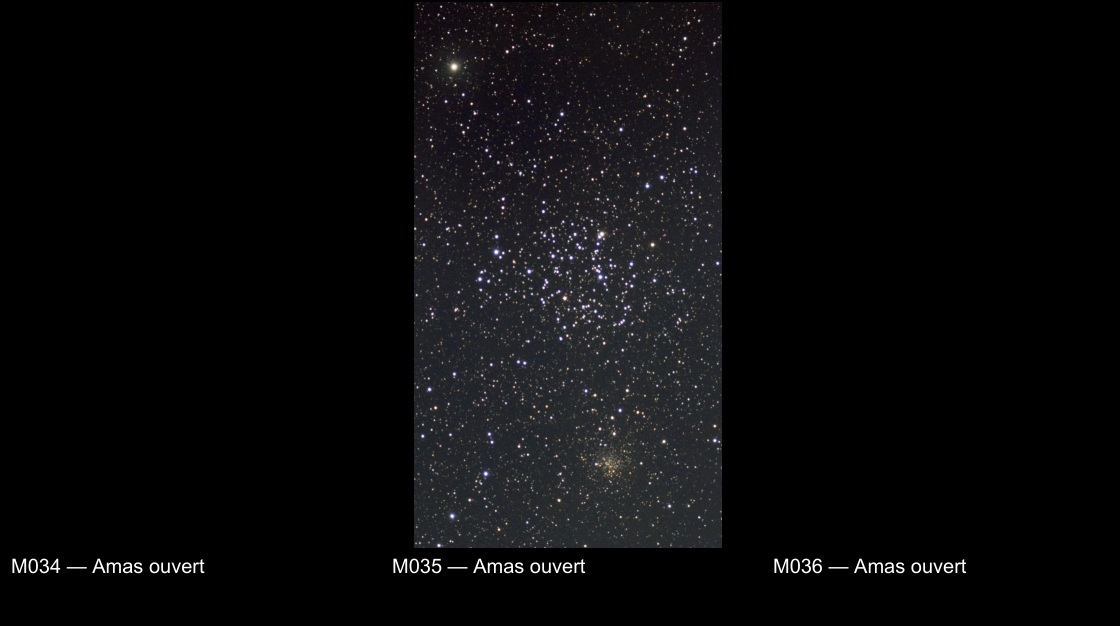
\includegraphics[width=.76\linewidth,height=48mm,keepaspectratio]{figures/affiche-messier-detail.jpg}
\caption{Détail de l'affiche effectivement produite. La position fixe des cases permet de distinguer une cible photographiée d'une cible qui reste à acquérir. Source : Steve Prud'Homme.}
\end{figure}

\subsection{GNU Astro Galery : retrouver la provenance d'une image}
Une galerie peut afficher une belle photographie après que sa date et sa durée d'exposition ont été perdues. GNU Astro Galery associe la consultation des images aux renseignements conservés dans les fichiers FITS, format astronomique qui réunit les données et un en-tête descriptif (Pence et coll., 2010). L'atelier illustre ce passage avec un répertoire consacré à M44, un en-tête FITS et une carte calculée centrée sur M102 (Prud'Homme, 2026a).

Le contrôle proposé consiste à choisir une exposition et à comparer la durée affichée avec la valeur de \texttt{EXPTIME} dans son en-tête. La même opération peut être répétée pour l'horodatage de début (\texttt{DATE-OBS}). La carte de M102 sert à situer le champ ; son centre calculé ne prouve à lui seul ni le pointage réel du télescope ni l'identité de l'objet photographié.

\subsection{GNU Astrolist : définir ce que veut dire « visible ce soir »}
À Laval, l'obstacle qui masque une partie de l'horizon rend une liste générique peu utile. La requête étudiée porte sur les objets Messier le 24 novembre 2026, entre 20~h et 22~h, pour un site situé à $45{,}57^\circ$ nord et $73{,}68^\circ$ ouest. Les azimuts admis vont de $15^\circ$ à $180^\circ$ et la hauteur minimale vaut $20^\circ$. Voici la commande de la version 0.11.0, à saisir sur une seule ligne (les retours facilitent la lecture).
\begin{otherlanguage}{english}
\begin{verbatim}
gnu-astrolist --date 2026-11-24 --time-range 20:00-22:00
  --timezone America/Toronto --lat 45.57 --lon -73.68
  --az-min 15 --az-max 180 --min-altitude 20
  --objects messier --limit 5 --offline
\end{verbatim}
\end{otherlanguage}
Le calcul a retenu vingt objets et en a affiché cinq. M42 offre le test le plus instructif : à 20~h, sa hauteur calculée est de $3{,}9^\circ$. Elle franchit le seuil vers 21~h~38 et atteint $23{,}1^\circ$ à 22~h. Sa présence dans la liste signifie donc qu'elle satisfait les critères pendant une partie du créneau. Le mode hors ligne utilise les données locales ; la table de rotation terrestre disponible dépassait sa période de validité. Ces valeurs arrondies servent à planifier une sortie. La météo et l'observation effective relèvent du carnet de terrain.

\subsection{GNU Astrophotography Recycle : examiner une trace}
Des poses individuelles écartées lors de l'empilement peuvent garder la trace d'un objet mobile. L'étude illustrée porte sur seize poses du Seestar S50. Le traitement rapproche une trace mesurée sur l'image de trajectoires prévues pour l'heure et le champ enregistrés. Les 935 lignes candidates produites pendant la recherche représentent des comparaisons à examiner. Plusieurs peuvent concerner la même pose ou le même objet.

Trois rapprochements sont qualifiés de plausibles dans le dossier : S03-03 avec KUIPER-00116, S03-08 avec STARLINK-1301 et S04-04 avec CENTISPACE-1 S13. Une trace faible, S04-01, a été écartée de cette sélection. Conserver ce dernier exemple rend la décision discutable au sens scientifique : un autre observateur peut retrouver le signal, examiner sa faiblesse et proposer une autre lecture. Les trois noms demeurent des hypothèses.
\begin{figure}[htbp]\centering
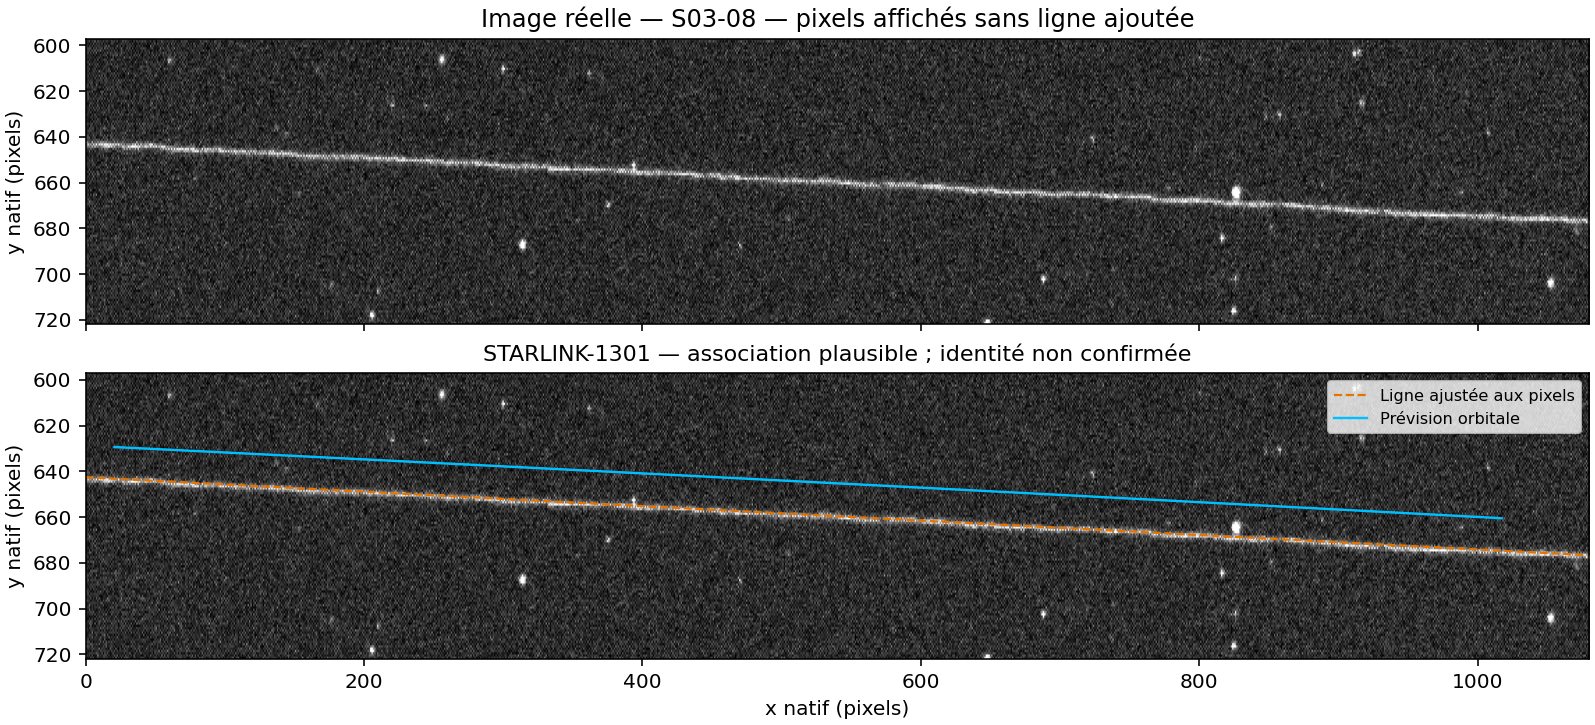
\includegraphics[width=.87\linewidth,height=64mm,keepaspectratio]{figures/recycle-s03-08.png}
\caption{Cas S03-08 du dossier illustré. La pose contient une trace ; son rapprochement avec STARLINK-1301 repose sur la comparaison avec une trajectoire calculée. Source : Steve Prud'Homme.}
\end{figure}

\section{Discussion : rendre le contrôle transmissible}
Les cas Messier et Astrolist révèlent deux ambiguïtés qu'un programme peut masquer derrière une sortie convaincante. Pour l'affiche, l'unité à compter est l'objet astronomique. Pour la soirée d'observation, il faut préciser si la cible doit rester visible tout le créneau ou seulement le traverser. Une consigne devient vérifiable lorsqu'elle contient un exemple dont on connaît l'issue : deux alias de la même galaxie doivent remplir une seule case ; une nébuleuse qui se lève en cours de soirée doit apparaître avec l'heure où elle devient accessible.

Le dialogue avec l'IA permet de préciser ces règles et d'obtenir rapidement un premier essai. L'atelier distingue la discussion d'une consigne, le travail sur des documents et l'intervention d'un agent de programmation sur le dépôt. Dans ce dernier cas, le membre peut examiner les différences entre deux versions et rejouer le même essai. Un \emph{commit} Git associe une révision à une modification identifiable. Le fichier \texttt{README.md} relie la version, les prérequis et la commande d'exemple ; la licence précise les conditions de réutilisation. Cette organisation rapproche le projet de pratiques communautaires documentées en astronomie par la collaboration Astropy (2022). Le corpus ne mesure ni les jetons consommés ni le temps gagné.

Pour la science citoyenne, l'exigence supplémentaire apparaît dans le quatrième cas. Partager la conclusion « satellite plausible » ne suffit pas à un second club pour la vérifier. Il lui faudrait aussi la pose originale, le site, l'heure et son incertitude, la solution de position du champ, les données orbitales datées et le critère de comparaison. Le corpus ne fournit pas de série de contrôle qui permettrait d'estimer un taux de fausses associations. Diviser trois par seize décrirait seulement le nombre de rapprochements retenus par rapport au nombre de poses, sans renseigner sur la fiabilité des identifications.

\section{Conclusion}
Dans cet atelier de club, le rôle décisif de l'observateur consiste à transformer son expérience du ciel en contrôles concrets : reconnaître deux noms pour un objet, relire un en-tête, dater le passage d'un seuil ou conserver une trace dont l'interprétation reste ouverte. Une suite possible serait de confier la même série de poses à un autre club avec les paramètres de calcul, puis de comparer les décisions prises indépendamment. Cet essai permettrait de mesurer la reproductibilité du classement présenté ici.

\section*{Ressources de la conférence}
\noindent\begin{minipage}{.20\linewidth}\centering
\qrcode[height=26mm]{https://github.com/steveprudhomme/atelier-vibe-coding-astronomie}
\end{minipage}\hfill\begin{minipage}{.76\linewidth}
Le code QR ouvre le dépôt de la conférence. La rubrique \emph{Ressources de la conférence} rassemble les diapositives, les notes du présentateur, la bibliographie BibTeX, le manuscrit et des articles scientifiques en accès libre.\\[3pt]
\url{https://github.com/steveprudhomme/atelier-vibe-coding-astronomie}
\end{minipage}

\section*{Références}
\nocite{ref07,ref18,ref19,ref20,ref21,ref23,articleAstropy,articleFits}
\bibliographystyle{atelier-uqam}
\bibliography{references,article/science}
\clearpage
\pdfbookmark[1]{Annexe A -- Diapositives intégrales}{annexe-diapos}
\section*{Annexe A. Diapositives intégrales}
Les pages suivantes reproduisent la présentation dans son ordre de projection, y compris les étapes successives des démonstrations, les schémas en grand format et la bibliographie. Le numéro affiché sur chaque diapositive est celui de l'atelier. Les signets du PDF permettent de passer directement à l'annexe B pour lire le texte correspondant du présentateur.
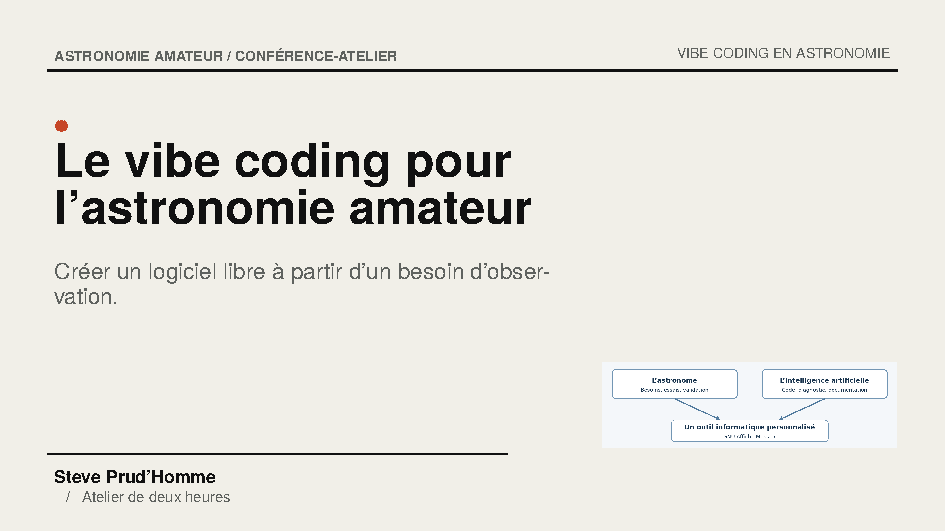
\includepdf[pages=-,fitpaper=true,pagecommand={}]{presentation.pdf}
\clearpage
\pdfbookmark[1]{Annexe B -- Notes intégrales du présentateur}{annexe-notes}
\section*{Annexe B. Notes intégrales du présentateur}
Les notes reproduites ci-après conservent le texte oral, les indications de durée, les consignes de projection, les légendes et les références du document de conférence. Les exemples chiffrés sur les offres commerciales sont ceux de la conférence.
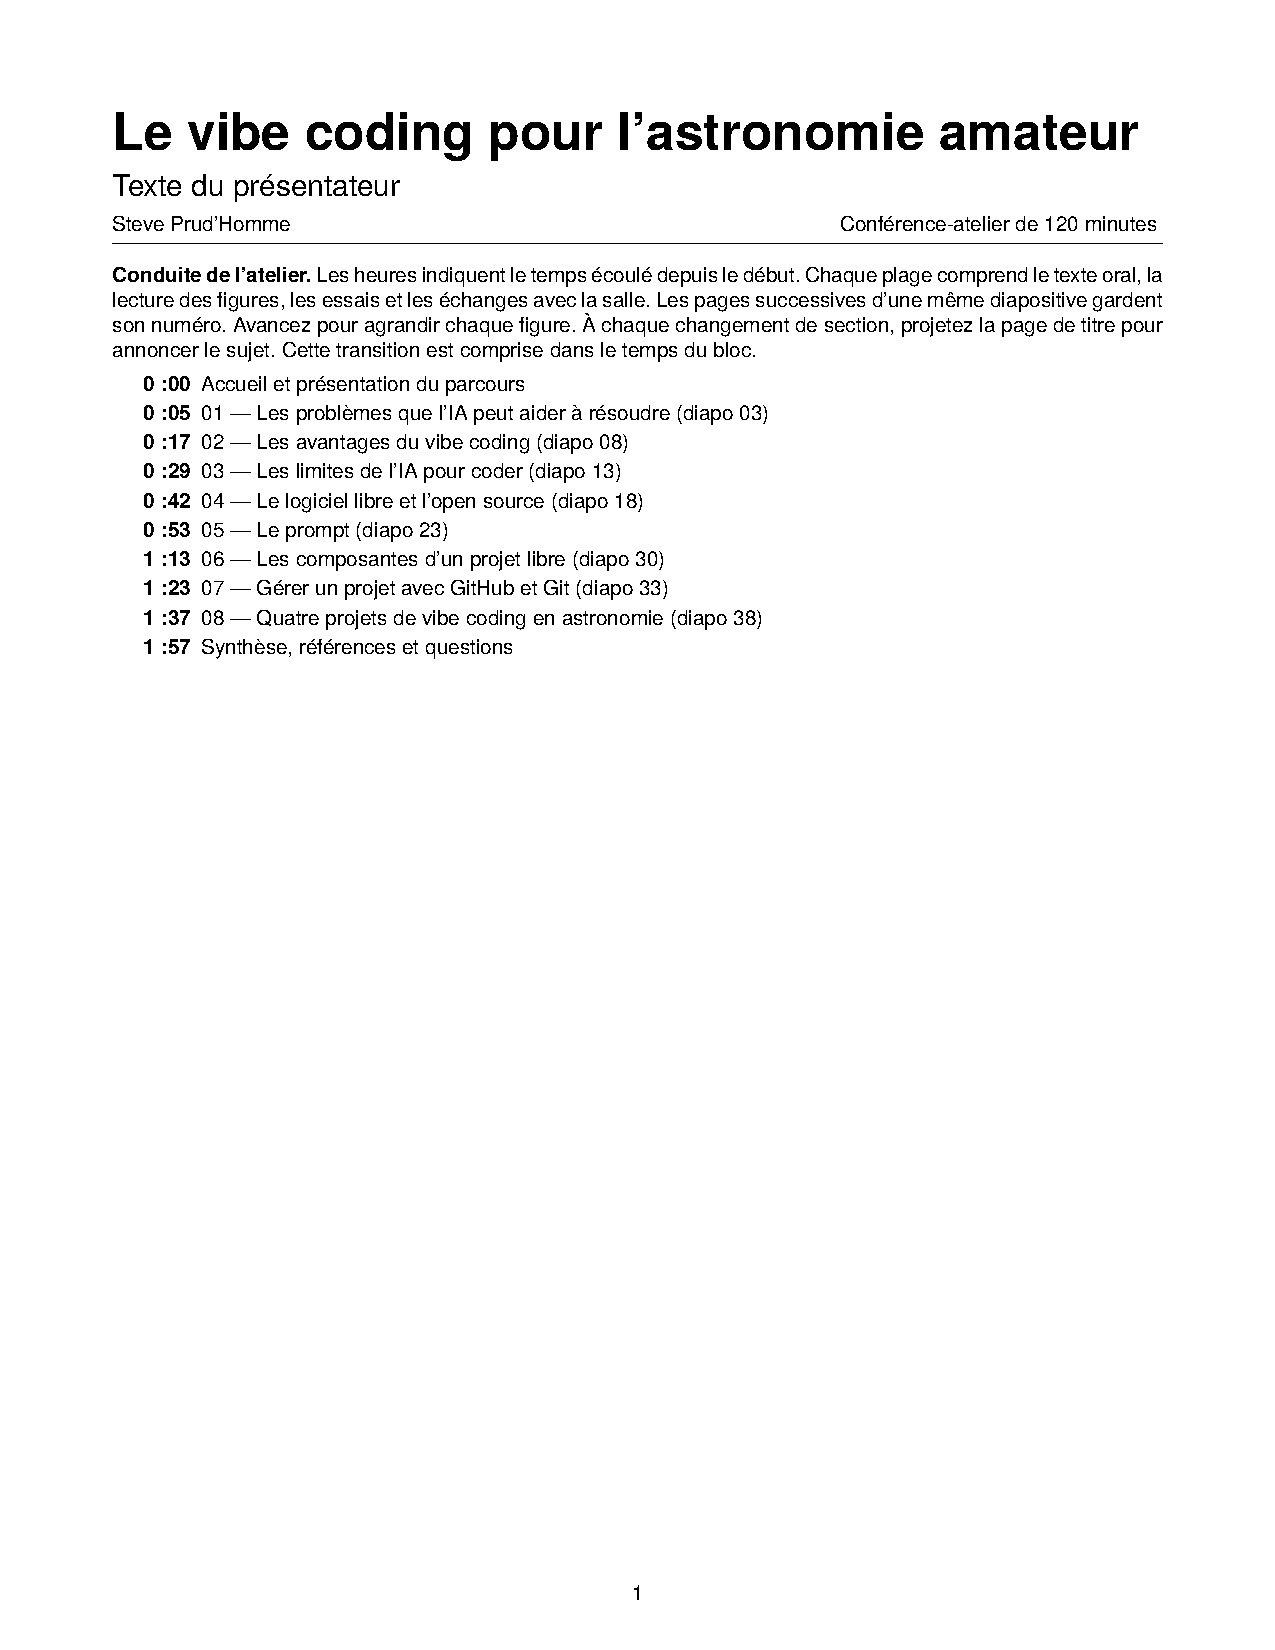
\includepdf[pages=-,fitpaper=true,pagecommand={}]{notes.pdf}
\end{document}
